\documentclass[11pt]{article}

\usepackage[T1]{fontenc}
\usepackage[margin=1in]{geometry}
\usepackage{amsmath}
\usepackage{graphicx}
\usepackage{booktabs}
\usepackage{tabularx}
\usepackage{array}
\usepackage{xcolor}
\usepackage{listings}
\usepackage{tikz}
\usepackage{microtype}
\usepackage[round,authoryear]{natbib}
\usepackage[hidelinks]{hyperref}

\usetikzlibrary{arrows.meta,positioning}

\definecolor{codebackground}{RGB}{248,248,248}
\definecolor{codecomment}{RGB}{55,105,55}
\definecolor{codekeyword}{RGB}{30,70,150}
\definecolor{codestring}{RGB}{145,55,55}

\lstdefinestyle{Rstyle}{
  language=R,
  backgroundcolor=\color{codebackground},
  basicstyle=\ttfamily\footnotesize,
  keywordstyle=\color{codekeyword},
  commentstyle=\color{codecomment},
  stringstyle=\color{codestring},
  numbers=left,
  numberstyle=\tiny\color{gray},
  numbersep=8pt,
  frame=single,
  rulecolor=\color{gray},
  breaklines=true,
  breakatwhitespace=false,
  showstringspaces=false,
  keepspaces=true,
  columns=fullflexible,
  tabsize=2,
  captionpos=b
}

\graphicspath{{figures/}{figures/experiment4/}}

\newcommand{\Btrue}{B_{\mathrm{true}}}
\newcommand{\Bconst}{B_{\mathrm{const}}}
\newcommand{\sigB}{\sigma_B}

\title{Recovering a Time-Varying Transmission Rate\\
with Simulation-Based Inference}
\author{Yixin Ma}
\date{Summer 2026}

\begin{document}

\maketitle

\begin{abstract}
Estimating a time-varying transmission rate from reported case data is challenging because epidemic transmission dynamics are stochastic and only partially observed. Within a partially observed Markov process framework, this report compares two representations of the transmission rate \(B(t)\): a latent Gamma-noise process that allows \(B(t)\) to vary over time and a constant-\(B\) formulation. Both models are fitted using the same likelihood-based inference framework. Particle filtering is used to approximate the likelihood and filtering distribution, while iterated filtering (IF2) is used to estimate the static parameters.

The comparison is evaluated using a simulation benchmark in which the prescribed deterministic transmission rate changes from \(B(t)=4\) before week~5 to \(B(t)=2\) from week~5 onward. Across 200 paired simulated data sets satisfying the acceptance criterion, the Gamma-noise fitting model is compared with a stochastic epidemic fitting model having a constant transmission rate. Recovery accuracy is measured using the root mean squared error (RMSE) between one ancestry-preserving sampled latent trajectory from the selected Gamma fit and the prescribed transmission-rate trajectory; the constant-model estimate is repeated over time. Under this benchmark, mean RMSE was 0.653 for Gamma-noise and 1.199 for constant-\(B\), with lower Gamma-noise RMSE in 195 of 200 paired data sets.
\end{abstract}

\tableofcontents
\clearpage

\section{Introduction}

Infectious disease outbreaks are commonly observed through univariate or multivariate time series of reported cases, such as the number of newly reported cases aggregated over a specified time interval. These data record when and how many cases were reported, but they do not directly reveal the underlying process by which infection spreads through a population. Mechanistic epidemic models connect the observed cases to changes in susceptible, infectious, and recovered populations by explicitly representing the dynamics of disease transmission \cite{breto2009mechanistic}. Partially observed Markov process (POMP) models provide a general framework for such models by separating two components: a latent Markov process describing the transmission dynamics and an observation process linking the latent states to the reported cases \cite{king2016pomp}.

Statistical inference for stochastic POMP models is generally difficult. Even when the static parameters and initial conditions are fixed, a stochastic model can generate many different latent epidemic trajectories. Evaluating the likelihood of the observed data requires integrating over these unobserved epidemic states and transmission histories, and the resulting likelihood therefore does not usually have a simple closed-form expression. Many statistical methods have been proposed for inference on POMP models \cite{breto2009mechanistic,king2016pomp}. These methods make it possible to use reported cases to infer epidemic processes and parameters that cannot be observed directly.

Within this framework, this report focuses on how to represent and infer a transmission rate that varies over time. The constant-$B$ POMP model assumes that the transmission rate remains fixed throughout the epidemic. In practice, the transmission rate may change with contact behavior, public-health interventions, and other conditions, while the transmission rate itself cannot be observed directly from reported cases \cite{bouman2024timevarying}. This report therefore incorporates Gamma noise into the process model and represents the transmission rate as a positive latent stochastic process \cite{breto2009mechanistic}. The Gamma-noise POMP model is then compared with the constant-$B$ POMP model to assess their ability to infer a time-varying transmission rate from reported cases.

This study is a simulation-based model comparison and a transmission-rate recovery study. Its central question is whether, under a prescribed piecewise truth in which the transmission rate decreases from 4 to 2 beginning at week 5, the Gamma-noise POMP model can recover the known time-varying transmission rate more accurately than the constant-$B$ POMP model. The experimental design contains three distinct POMP models. A data-generating POMP combines the prescribed transmission-rate path with a stochastic SIR transmission process and a negative-binomial observation model to generate reported cases. The same reported cases are then supplied to two fitting POMPs. The Gamma-noise POMP model treats the transmission rate as a time-varying latent stochastic process, whereas the constant-$B$ POMP model estimates a single transmission-rate parameter for the entire epidemic. Neither fitting model is given the true transmission-rate path or the location of its change point.

For a fixed set of parameter values, the particle filter is used to estimate the likelihood of the observed data and obtain filtering summaries of the transmission rate and other latent states \cite{gordon1993particle,king2016pomp}. Iterated filtering (IF2) uses this particle-filtering framework to search the static parameter space of each fitting model \cite{ionides2015if2}. These algorithms support statistical inference for the model comparison; they are not components of the epidemic models themselves. The inferential performance of the two models is evaluated primarily by comparing the estimated transmission rates with the known truth using recovery error and root mean squared error (RMSE).

This report investigates the ability of the Gamma-noise POMP model to infer a time-varying transmission rate and compares its performance with that of the constant-$B$ POMP model in a controlled simulation study. The results show that, when the prescribed transmission rate decreases from 4 to 2, the Gamma-noise POMP model recovers the transmission-rate path more accurately and produces a lower RMSE. Section~2 defines the stochastic epidemic process, the observation process, and the two transmission models. Section~3 introduces the particle filter and IF2 used for inference, together with the measures used to evaluate recovery performance. Sections~4--6 present the simulation design, the results, and their interpretation.

\section{Model}
\label{sec:model}

\subsection{Three POMP models}

Experiment~4 uses one data-generating POMP and two fitting POMPs
(Figure~\ref{fig:model-hierarchy}).  All three models contain the same
stochastic epidemic transitions and negative-binomial observation process.
They differ only in the source of the transmission rate used by the epidemic
process.  The data-generating model uses a prescribed deterministic path
\(\Btrue(t)\); the Gamma-noise fitting model includes \(B(t)\) as a positive
latent stochastic state; and the constant-\(B\) fitting model uses one positive
static parameter \(\Bconst\).

This separation makes the comparison interpretable.  The generator defines
the target against which recovery is measured, whereas the two fitting models
define alternative explanations of the same observations.  Calling the
prescribed path deterministic refers only to its transmission-rate input: the
epidemic trajectory and the reported cases generated from it are random.  In
the same way, calling the comparator constant refers only to its transmission
rate; its epidemic and observation processes remain stochastic.

\begin{figure}[htbp]
\centering
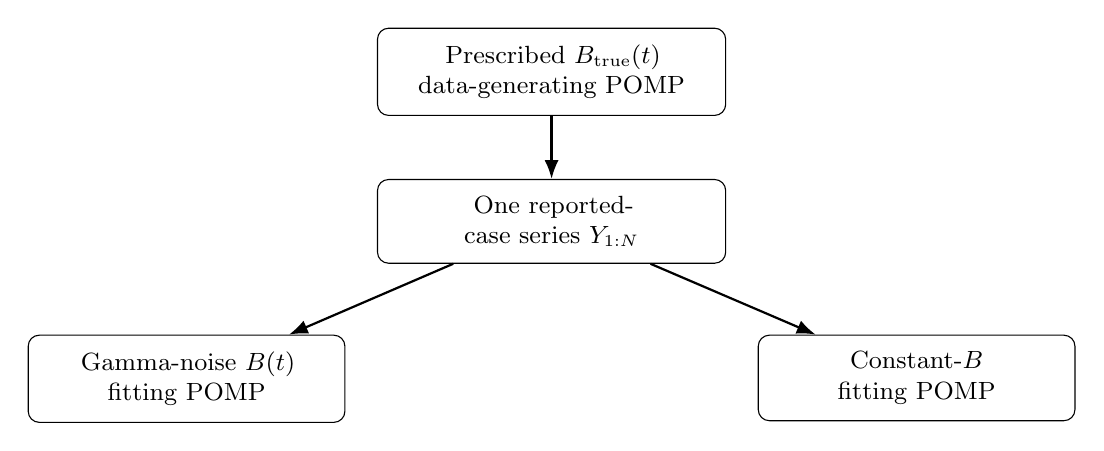
\begin{tikzpicture}[
  node distance=0.8cm and 1.0cm,
  box/.style={
    draw,
    rounded corners,
    align=center,
    minimum height=0.9cm,
    text width=4.0cm,
    inner sep=6pt,
    font=\small
  },
  fitbox/.style={
    draw,
    rounded corners,
    align=center,
    minimum height=0.9cm,
    text width=3.6cm,
    inner sep=6pt,
    font=\small
  },
  arrow/.style={-{Latex[length=2.4mm]},thick}
]
\node[box] (generator)
  {Prescribed \(B_{\mathrm{true}}(t)\)\\data-generating POMP};
\node[box,below=of generator] (data)
  {One reported-case series \(Y_{1:N}\)};
\node[fitbox,below left=0.9cm and 0.4cm of data] (gamma)
  {Gamma-noise \(B(t)\)\\fitting POMP};
\node[fitbox,below right=0.9cm and 0.4cm of data] (constant)
  {Constant-\(B\)\\fitting POMP};
\draw[arrow] (generator) -- (data);
\draw[arrow] (data) -- (gamma);
\draw[arrow] (data) -- (constant);
\end{tikzpicture}
\caption{Three-model design.  Each simulated case series is supplied unchanged
to both fitting POMPs.}
\label{fig:model-hierarchy}
\end{figure}

Immediately before measurement at observation time \(t_n\), the Gamma-noise
state is
\[
X_n^{(G)}
=\{S(t_n),I(t_n),R(t_n),H(t_n),B(t_n)\}.
\]
The data-generating and constant-\(B\) states omit the dynamic transmission
component:
\[
X_n^{(D)}=X_n^{(C)}
=\{S(t_n),I(t_n),R(t_n),H(t_n)\}.
\]
The variable \(H\) is an incidence accumulator.  It records infections since
the previous observation and is reset after the corresponding measurement is
generated.

\subsection{Stochastic SIR process}

Let \(S_k\), \(I_k\), and \(R_k\) be the susceptible, infectious, and recovered
counts at Euler time \(t_k\), with step length \(\Delta t\).  Write
\(B_k^{\mathrm{use}}\) for the transmission value supplied by the relevant
model.  The one-step infection and recovery probabilities are
\begin{align}
p_{SI,k}
&=1-\exp\left(-B_k^{\mathrm{use}}I_k\Delta t/N\right),&
p_{IR,k}
&=1-\exp\left(-\mu_{IR}\Delta t\right).
\end{align}
Conditional on the current state, the event counts are
\begin{align}
\Delta N_{SI,k}
&\sim\operatorname{Binomial}(S_k,p_{SI,k}),&
\Delta N_{IR,k}
&\sim\operatorname{Binomial}(I_k,p_{IR,k}).
\end{align}
The factor \(B_k^{\mathrm{use}}I_k/N\) is the per-susceptible infection
hazard.  The exponential conversion gives the probability of infection over
the finite step \(\Delta t\), while the recovery probability is derived from
the constant recovery hazard \(\mu_{IR}\).  This construction keeps both
probabilities in \([0,1]\) and lets the same transition equations accept any
of the three transmission inputs.
The state then changes according to
\begin{align}
S_{k+1} &= S_k-\Delta N_{SI,k},\\
I_{k+1} &= I_k+\Delta N_{SI,k}-\Delta N_{IR,k},\\
R_{k+1} &= R_k+\Delta N_{IR,k},\\
H_{k+1} &= H_k+\Delta N_{SI,k}.
\end{align}
Thus \(S_k+I_k+R_k=N\), while \(H_k\) records events rather than people and is
excluded from the population total.  The binomial draws make the epidemic
process stochastic even when \(B_k^{\mathrm{use}}\) is deterministic or
constant.

The accumulator bridges the process and observation time scales.  The SIR
state is updated every Euler step, but cases are observed only once per day.
Summing \(\Delta N_{SI,k}\) into \(H\) preserves all infections between two
measurements; resetting \(H\) after measurement prevents the same infection
from contributing to more than one reported count.

\subsection{Observation model}

Let \(H_n\) be the infections accumulated during
\((t_{n-1},t_n]\), immediately before reset, and let \(Y_n\) be the reported
case count.  Reported cases depend on incidence \(H_n\), not on the number
infectious at one instant.  The model is
\begin{equation}
Y_n\mid H_n
\sim
\operatorname{NegBin}
\left(\text{mean}=\rho H_n,\ \text{size}=k\right),
\label{eq:measurement}
\end{equation}
with
\[
\operatorname{E}(Y_n\mid H_n)=\rho H_n,
\qquad
\operatorname{Var}(Y_n\mid H_n)
=\rho H_n+\frac{(\rho H_n)^2}{k}.
\]
Here \(\rho\) controls the expected reported fraction and \(k\) controls
overdispersion around that conditional mean.  The observation model does not
feed reports back into the epidemic: \(Y_n\) is generated from \(H_n\), after
which the latent SIR process continues from its current state.
This negative-binomial variation is observation noise conditional on latent
incidence.  It is distinct from the binomial demographic variation in the SIR
transitions.

\subsection{Transmission-rate models}

\paragraph{Gamma-noise model.}
The Gamma-noise fitting POMP initializes \(B(0)=B_0>0\).  At each Euler step it
draws
\begin{equation}
B_{k+1}\mid B_k
\sim
\operatorname{Gamma}
\left(
  \text{shape}=\frac{1}{\sigB^2\Delta t},
  \ \text{scale}=B_k\sigB^2\Delta t
\right),
\label{eq:gamma-update}
\end{equation}
and uses the updated value \(B_{k+1}\) immediately in the infection
probability.  The two static transmission parameters are \(B_0\) and
\(\sigB\); the sequence \(B(t)\) remains latent.

For the shape--scale parameterization in
Equation~\ref{eq:gamma-update},
\begin{align}
\operatorname{E}(B_{k+1}\mid B_k)
&=B_k,\\
\operatorname{Var}(B_{k+1}\mid B_k)
&=B_k^2\sigB^2\Delta t.
\end{align}
The transition therefore has zero conditional drift and one-step conditional
coefficient of variation \(\sigB\sqrt{\Delta t}\).  Larger \(\sigB\) permits
greater relative movement between adjacent process times.  Because the Gamma
distribution has positive support, \(B(t)\) remains positive.  When time is
measured in weeks, \(B(t)\) has units \(\mathrm{week}^{-1}\) and \(\sigB\)
has units \(\mathrm{week}^{-1/2}\).

Zero conditional drift does not force a realized path to remain flat.  A draw
can move above or below the current value, and successive innovations can
accumulate into a sustained change.  Conversely, the transition contains no
preferred change point, downward trend, or mean-reversion level.  Evidence for
a decline must therefore enter through the observed cases during filtering.
The role of \(\sigB\) is specifically to regulate local relative process
variation; it is not a reporting-dispersion parameter and it is not an IF2
search perturbation.

\paragraph{Prescribed data-generating rate.}
The data-generating POMP sets
\[
B_k^{\mathrm{use}}=\Btrue(t_k).
\]
This path is fixed by the simulation design rather than drawn from
Equation~\ref{eq:gamma-update}.  The generated epidemic and reports are still
random because their binomial transitions and negative-binomial measurements
remain stochastic.  Section~\ref{sec:design} gives the prescribed path and
parameter values.

\paragraph{Constant-\(B\) model.}
The constant fitting POMP estimates one positive parameter \(\Bconst\) and
sets
\[
B_k^{\mathrm{use}}=\Bconst
\]
throughout the epidemic.  It has no latent transmission-rate state, but it
retains the same stochastic SIR and observation processes as the other two
POMPs.

The scientific dependence common to all three models is
\[
B(t)
\longrightarrow
\text{infection hazard}
\longrightarrow
\text{new infections}
\longrightarrow
H_n
\longrightarrow
Y_n.
\]
The Gamma-noise model adds stochastic variation at the first link.  Particle
filtering and IF2, introduced next, are computational tools for inference and
do not add scientific transitions to this chain.

Five sources of variation should therefore be kept separate.  Gamma process
noise moves the latent transmission rate only in the Gamma-noise fitting POMP;
binomial demographic noise moves the epidemic counts in all three POMPs; and
negative-binomial observation noise moves reported cases around latent
incidence.  Particle-filter Monte Carlo error is numerical approximation error
from using finitely many particles, while IF2 perturbations are temporary
optimization devices.  The last two affect inference but are not components
of the scientific epidemic model.

\section{Inference and evaluation}
\label{sec:method}

\subsection{Likelihood and maximum-likelihood estimation}

The observed case series does not reveal the epidemic states or, in the
Gamma-noise model, the transmission-rate path.  The observed-data likelihood
therefore averages over all latent state histories compatible with a fixed
parameter vector.  That integral is not available analytically for these
nonlinear stochastic POMP models.  The inferential target is the maximum
likelihood estimate
\begin{equation}
\widehat{\theta}
=
\arg\max_{\theta}\ell(\theta;y_{1:N}).
\label{eq:mle}
\end{equation}
The model-specific static transmission parameters are
\[
\theta_G=(B_0,\sigB),
\qquad
\theta_C=(\Bconst).
\]
The nuisance parameters \(\mu_{IR},N,\rho,k\) and the initial epidemic state
are fixed in this benchmark.  In particular, the latent sequence \(B(t)\) is
not optimized as an unrelated parameter at every time point; it is integrated
over according to the Gamma transition in Equation~\ref{eq:gamma-update}.

\subsection{Particle filtering}

For a fixed parameter vector, a particle filter propagates many possible
latent states through the process model, weights them according to each new
reported count, and resamples states that better explain the observations.
These weighted particles approximate both the observed-data likelihood and
the filtering distribution of the latent state given reports through the
current observation time \citep{gordon1993particle,king2016pomp}.  The analysis
uses the implementation in the \texttt{pomp} package
\citep{king2025pomp64}.

At an observation time, weighting favors particles whose accumulated
incidence makes the reported count plausible; resampling then concentrates
subsequent computation on those histories without collapsing the scientific
model to a single path.  Because only finitely many particles are used, two
independent filters at the same parameter vector need not return identical
likelihood estimates or sampled latent histories.  This particle-filter Monte Carlo
variation is reduced by increasing the particle population and is separate
from every biological or reporting source of randomness in Section~\ref{sec:model}.

\subsection{IF2 estimation}

Iterated filtering (IF2) connects particle filtering to the optimization in
Equation~\ref{eq:mle} \citep{ionides2015if2}.  IF2 repeatedly applies a particle
filter to an extended parameter--state system.  Artificial perturbations allow
the static-parameter particles to explore the likelihood surface, while
observation weighting and resampling favor parameter--state combinations that
better explain the data.  A cooling schedule reduces the perturbation scale
across iterations, producing an approximate maximum likelihood estimate.
Multiple starting points broaden the search but do not guarantee that the
global maximum has been found.

In the implemented search, each starting point underwent a fixed sequence of
600 IF2 iterations.  The decreasing perturbations turn the early iterations
into relatively broad exploration and the later iterations into a more local
search.  Candidate endpoints were not ranked using the final IF2 trace value
alone: five independent ordinary particle filters reevaluated each endpoint
after perturbations had been removed.  If \(\ell_{dsj}\) is the log-likelihood
estimate for data set \(d\), start \(s\), and evaluation \(j\), the ranking
summary was
\begin{equation}
\widetilde\ell_{ds}
=
\log\left\{\frac{1}{5}\sum_{j=1}^{5}\exp(\ell_{dsj})\right\},
\label{eq:logmeanexp}
\end{equation}
computed numerically with \texttt{pomp::logmeanexp}.  Thus the averaging occurs
on the likelihood scale.  It is neither an arithmetic mean of log likelihoods
nor a mean of the latent transmission trajectories.  The endpoint with the
largest finite \(\widetilde\ell_{ds}\) was selected as the best fit.  This
separates parameter search from the final comparison as far as the finite
computation allows.

IF2 perturbations are algorithmic and disappear from the focal model after
optimization.  They are distinct from Gamma process noise, which governs the
scientific evolution of latent \(B(t)\) at the fitted value of \(\sigB\).
Appendix~\ref{app:implementation} records the starting values, particle counts,
perturbation scales, cooling, and selection details.

\subsection{Transmission-rate recovery}

For paired data set \(d\), the selected Gamma parameters were passed to one
final 50,000-particle filter with trajectory ancestry retained.  The
\texttt{filter\_traj()} function then extracted one internally consistent
latent history,
\begin{equation}
\widehat B^{(G)}_d(t_{0:N})
=B^{*}_d(t_{0:N};\widehat\theta_{G,d}),
\label{eq:bhat}
\end{equation}
where the superscript \(*\) denotes the sampled history rather than a posterior
or filtering mean.  Because its ancestry is traced through the final particle
population, this is a finite-particle, plug-in-parameter approximation to a
smoothing trajectory conditional on the complete reported series.  It is not
an exact posterior draw, an uncertainty interval, or a separately optimized
value of \(B\) at each time.  The value at \(t_0\) is retained only for display;
all recovery metrics use the 70 observation times \(t_1,\ldots,t_N\).

The constant-model estimator is the selected static value repeated over those
same observation times,
\[
\widehat B^{(C)}_d(t_n)=\widehat B_{\mathrm{const},d}.
\]
Both models are therefore represented by one observation-time trajectory
before comparison, even though the constant trajectory necessarily repeats a
single value.  No filtering mean enters the Experiment~4 recovery metrics.
For model \(m\in\{G,C\}\), the primary task-level outcome is
\begin{equation}
\operatorname{RMSE}^{(m)}_d
=
\sqrt{
\frac{1}{N_{\mathrm{obs}}}
\sum_{n=1}^{N_{\mathrm{obs}}}
\left[
\widehat B^{(m)}_d(t_n)-\Btrue(t_n)
\right]^2
}.
\label{eq:rmse}
\end{equation}
This definition compares like observation times within each paired data set.
Each data set contributes one RMSE per model and therefore one within-pair
difference.  Averaging these task-level RMSE values gives equal weight to the
200 accepted epidemics, rather than allowing a data set with more cases to
dominate the summary.  Squaring before averaging also prevents early
underestimation and late overestimation from canceling.

Secondary summaries describe signed recovery error.  The task-level mean error
averages \(\widehat B^{(m)}_d(t_n)-\Btrue(t_n)\) over all observation times;
its absolute value measures overall displacement without allowing the final
sign to determine magnitude.  Segment-specific signed errors average the same
quantity before and after week~5.  Post-fitting particle-filter likelihoods
provide an additional same-data fitting diagnostic, but they are neither
penalized nor evaluated on held-out observations and are not treated as a
formal model-selection test.

\section{Simulation design}
\label{sec:design}

Experiment~4 is a paired recovery comparison.  For each task, the
data-generating POMP simulates an epidemic and reported cases once.  The
resulting observation times and case counts are saved and supplied unchanged
to the Gamma-noise and constant-\(B\) fitting POMPs.  Pairing removes
between-data-set variation from the model contrast: both fits must explain the
same realized epidemic reports.

Within a task, the deterministic transmission path drives a new stochastic
SIR realization, the accumulator records infections between daily
observations, and the negative-binomial model produces one case count at each
observation time.  Only these observation times and counts enter the two
fitting workflows.  The unobserved generating states are retained for
evaluation but are not supplied to IF2 or to the final filters.

The data-generating transmission path is
\begin{equation}
\Btrue(t)
=
\begin{cases}
4, & 0\leq t<5,\\[3pt]
2, & 5\leq t\leq10,
\end{cases}
\qquad \text{\(t\) in weeks.}
\label{eq:truth}
\end{equation}
This path is deterministic.  Neither fitting model receives
\(\Btrue(t)\), the values in Equation~\ref{eq:truth}, or the week-5 change
point.  The principal settings are summarized in
Table~\ref{tab:settings}.

The 70 daily observations span the ten-week horizon; the scheduled
observation at week~5 is evaluated under the post-change rate.  The Euler grid
is finer than the observation grid, with approximately four
process updates between successive daily measurements.  Fixing the recovery,
reporting, population, and initial-state quantities at their generating values
makes this a focused transmission-recovery experiment: it avoids adding
nuisance-parameter confounding to the primary comparison.

\begin{table}[htbp]
\centering
\caption{Experiment~4 simulation settings.}
\label{tab:settings}
\begin{tabularx}{0.88\textwidth}{>{\raggedright\arraybackslash}p{0.43\textwidth}X}
\toprule
Setting & Value \\
\midrule
Paired accepted data sets & 200 \\
Acceptance criterion & \(\max(H)>20\) \\
Duration & 10 weeks \\
Observation schedule & 70 daily observations, \(1/7,\ldots,10\) weeks \\
Euler step & \(\Delta t=1/30\) week \\
Prescribed transmission path & \(4\) before week~5; \(2\) from week~5 onward \\
Population size & \(N=10000\) \\
Recovery rate & \(\mu_{IR}=3~\mathrm{week}^{-1}\) \\
Reporting fraction & \(\rho=0.5\) \\
Negative-binomial size & \(k=10\) \\
Initial state & \(S(0)=9990,\ I(0)=10,\ R(0)=H(0)=0\) \\
\bottomrule
\end{tabularx}
\end{table}

The acceptance rule conditions the comparison on simulated outbreaks with
more than 20 accumulated infections in at least one observation interval.
Consequently, the reported recovery results describe accepted outbreaks under
these settings rather than all trajectories that the data-generating POMP
could produce.  Experiments~1--3 were developmental steps used to build and
calibrate the workflow; only Experiment~4 supplies the main scientific
evidence.  Their roles are summarized in
Appendix~\ref{app:developmental}.

\section{Results}
\label{sec:results}

\subsection{Primary recovery result}

The Gamma-noise model recovered the prescribed transmission path more
accurately than the constant-\(B\) model on the primary outcome.  Mean
task-level RMSE was 0.653 for Gamma-noise and 1.199 for constant-\(B\).
Gamma-noise had lower RMSE in 195 of 200 paired data sets (97.5\%).  The
task-by-task comparison in Figure~\ref{fig:paired-rmse} shows that the advantage
was widespread rather than being driven by a small subset of simulated
epidemics.

Relative to the constant-model mean, the difference corresponds to an
approximately 45.5\% reduction in mean RMSE.  The five reversals of the paired
ordering are visible above the equality line and prevent interpreting the
result as uniform across all accepted realizations.  The scatter also shows
variation in absolute recovery difficulty, as expected from stochastic
epidemic, reporting, and sampled-trajectory variation.

\begin{figure}[htbp]
\centering

\includegraphics[width=0.68\textwidth]{experiment4/04_paired_RMSE_scatter.pdf}
\caption{Paired RMSE calculated from the sampled Gamma trajectory and repeated
constant estimate for the same 200 accepted data sets.  Points below the
diagonal favor Gamma-noise.}
\label{fig:paired-rmse}
\end{figure}

Table~\ref{tab:errors} places the primary result beside the secondary
signed-error summaries.

\begin{table}[htbp]
\centering
\caption{Mean task-level recovery summaries across 200 paired data sets.}
\label{tab:errors}
\begin{tabular}{lrr}
\toprule
Quantity & Gamma-noise & Constant-\(B\) \\
\midrule
RMSE & 0.653 & 1.199 \\
Absolute task-level mean error & 0.229 & 0.606 \\
Signed mean error, \(t<5\) & -0.086 & -0.424 \\
Signed mean error, \(t\geq5\) & 0.008 & 1.576 \\
\bottomrule
\end{tabular}
\end{table}

\subsection{Secondary recovery summaries}

The mean absolute task-level mean error was 0.229 for Gamma-noise and 0.606
for constant-\(B\).  Gamma-noise had the smaller value in 177 of 200 data sets.
The segment-specific errors explain the main weakness of a single static rate.
Before week~5, mean signed error was \(-0.086\) for Gamma-noise and \(-0.424\)
for constant-\(B\).  From week~5 onward, the corresponding errors were 0.008
and 1.576.  The large positive constant-\(B\) error after the change indicates
that one fitted rate remained well above the prescribed value of 2.

The signed errors also show why the primary RMSE and the absolute mean error
answer different questions.  A constant estimate between 2 and 4 can be too
low in the first regime and too high in the second; averaging those signed
errors permits partial cancellation.  RMSE retains both discrepancies, while
the segment summaries reveal their direction.  Gamma-noise reduced both the
post-change overshoot and the overall displacement, although it did not
produce zero mean error in either segment.

Post-fitting likelihoods gave consistent supporting evidence: mean
particle-filter log likelihood was \(-191.08\) for Gamma-noise and \(-209.23\)
for constant-\(B\), and the saved paired difference favored Gamma-noise in 199
of 200 tasks.  This same-data, unpenalized comparison is a descriptive fitting
diagnostic rather than a formal model-selection test.  The error-distribution
and likelihood-difference figures are retained in
Appendix~\ref{app:diagnostics}.

These results summarize one sampled Gamma trajectory per accepted outbreak
under the specified benchmark.  They do not compare filtering means,
uncertainty intervals, repeated trajectory draws, or performance under other
transmission paths.

\section{Discussion}
\label{sec:discussion}

\subsection{Why the Gamma-noise model performed better}

The prescribed epidemic contains two transmission regimes, but the
constant-\(B\) model must explain both with one compromise value.  That
restriction produces a fitted rate that is too low before the change and much
too high afterward.  The Gamma-noise model can instead shift probability
toward lower latent \(B(t)\) paths as post-change reports arrive.  This
adaptation explains both its lower overall RMSE and its much smaller
post-change signed error.

The Gamma transition does not encode the true week-5 boundary or a
deterministic downward trend.  Its conditional mean equals the current rate,
so the fitted decrease emerges through conditioning on the observations:
particle paths that better explain the later reports receive more weight.
The comparison therefore shows the value of allowing transmission to change;
it does not show that a Gamma process generated the prescribed discontinuity.

\subsection{What the result means}

The lower RMSE in 195 of 200 paired data sets shows that a positive latent-rate
model usually recovered this imposed change more accurately than a static-rate
model when both were fitted to the same noisy case series.  Because all three POMPs
retain the same stochastic SIR and observation components, the contrast is
attributable to how the fitting models represent transmission rather than to
one model being stochastic and the other deterministic.

The secondary summaries support the same interpretation while measuring
different features of error.  Absolute task-level mean error can benefit from
cancellation between early negative and later positive errors, so it need not
rank models identically to RMSE in every data set.  The post-fitting likelihood
pattern shows that the more flexible model usually assigned higher likelihood
to the fitted observations, but it does not account for model complexity or
out-of-sample performance.

\subsection{Limitations and next step}

Three limitations define the scope of the conclusion:
\begin{itemize}
\item \emph{Benchmark scope.}  The experiment studies one abrupt path over ten
weeks and conditions on outbreaks satisfying \(\max(H)>20\).  Other change
sizes, timings, smooth trajectories, or weaker outbreaks may yield different
recovery behavior.
\item \emph{Fixed nuisance parameters.}  The recovery rate, reporting model,
population size, and initial state are fixed at their generating values.
Applied analyses must confront confounding between these quantities and
transmission, especially when a flexible \(\sigB\) can absorb other
misspecification.
\item \emph{Finite optimization.}  IF2 uses a finite particle population,
cooling schedule, and set of starting points.  The Gamma model received nine
starts and the constant model six, so the experiment does not establish equal
computational budgets or guarantee global maximization.
\item \emph{Single sampled trajectory.}  Recovery metrics use one
ancestry-preserving latent path from the final filter for each Gamma fit.  They
therefore include finite-particle and path-sampling variation and should not be
interpreted as posterior-mean error or as a summary of trajectory uncertainty.
Repeated trajectory extraction would be needed to quantify that additional
uncertainty.
\end{itemize}

A useful next comparison would replace local Gamma innovations with a smooth
basis representation,
\[
\log B(t)=\sum_{q=1}^{Q}c_q\phi_q(t),
\]
where \(\phi_q(t)\) are B-spline basis functions
\citep{bouman2024timevarying}.  Such a model would trade local stochastic
adaptation for a globally smooth trajectory whose flexibility depends on the
number and placement of knots and on regularization.  Because smoothing can
blur an abrupt change, the basis dimension and penalty would need to be
prespecified and evaluated in a new simulation study.  The next scientific
question is therefore whether Gamma noise or a controlled smooth-basis model
recovers a wider range of plausible transmission paths more reliably.


\clearpage
\appendix
\section{Developmental experiments}
\label{app:developmental}

Experiments~1--3 developed the modeling and computational workflow but do not
contribute numerical evidence to the main comparison.

\begin{table}[htbp]
\centering
\small
\caption{Developmental progression to Experiment~4.}
\begin{tabularx}{\textwidth}{
  >{\raggedright\arraybackslash}p{0.12\textwidth}
  >{\raggedright\arraybackslash}p{0.25\textwidth}
  >{\raggedright\arraybackslash}p{0.27\textwidth}
  >{\raggedright\arraybackslash}X}
\toprule
Experiment & Purpose & Why developmental & Link to Experiment~4 \\
\midrule
1
& Construct and illustrate the Gamma-noise model under constant and
piecewise transmission scenarios.
& Each scenario used one simulated epidemic and primarily examined model
construction and starting-value sensitivity.
& Established the basic latent-rate recovery workflow. \\
2
& Exercise a high-particle, multi-start Gamma-noise fitting workflow.
& The workflow was applied to one fixed simulated data set.
& Established the repeated-fitting workflow. \\
3
& Evaluate Gamma-noise recovery across 200 tasks with
\(N_{\mathrm{mif}}=100\).
& Its lower-iteration analysis was superseded for final numerical claims.
& Motivated the \(N_{\mathrm{mif}}=600\) paired comparison. \\
4
& Compare Gamma-noise and constant-\(B\) recovery on shared data.
& Main experiment rather than developmental evidence.
& Supplies all numerical results in the main text. \\
\bottomrule
\end{tabularx}
\end{table}

\section{Supporting diagnostics}
\label{app:diagnostics}

\subsection{Recovery-error distributions}

Figure~\ref{fig:error-distributions} shows the distribution of task-level
signed mean errors underlying the secondary summaries in
Table~\ref{tab:errors}.  It is retained as supporting evidence rather than as a
second presentation of the primary RMSE result.

\begin{figure}[htbp]
\centering

\includegraphics[width=0.94\textwidth]{experiment4/03_mean_error_distributions.pdf}
\caption{Task-level signed mean errors across 200 paired data sets.  Dashed
lines mark zero and dotted lines mark panel means.}
\label{fig:error-distributions}
\end{figure}

\subsection{Post-fitting likelihood diagnostic}

Figure~\ref{fig:likelihood-difference} displays the paired same-data
particle-filter likelihood differences.  Positive values favor Gamma-noise
numerically, but the diagnostic is unpenalized and is not based on held-out
observations.

\begin{figure}[htbp]
\centering
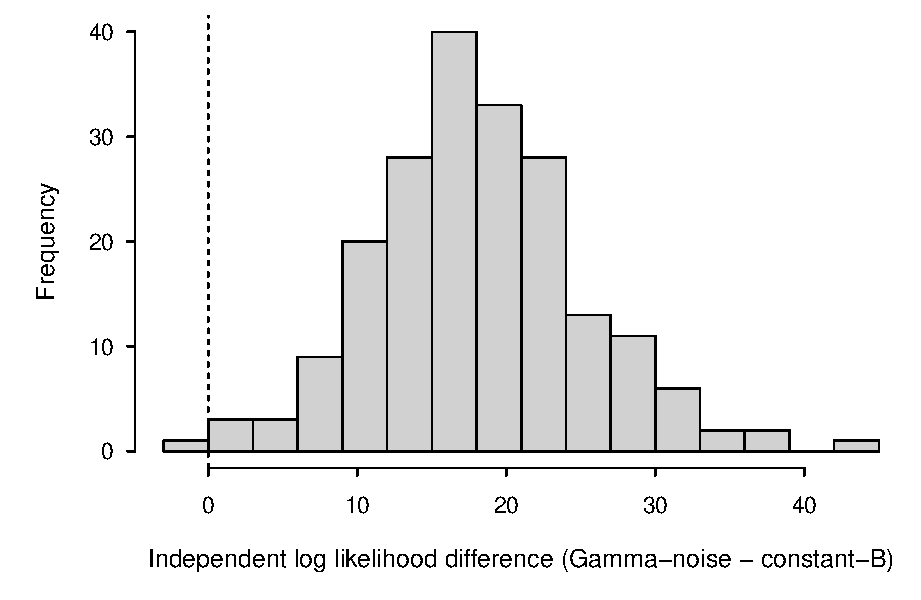
\includegraphics[width=0.82\textwidth]{experiment4/06_independent_loglik_difference.pdf}
\caption{Gamma-noise minus constant-\(B\) post-fitting log-likelihood
differences for 200 paired data sets.}
\label{fig:likelihood-difference}
\end{figure}

\subsection{Available convergence diagnostics}
\label{app:convergence}

Complete IF2 traces were saved for tasks 1, 50, 100, 150, and 200.  The files
\begin{itemize}
\item \path{figures/experiment4/convergence/gamma_convergence_diagnostics.pdf},
\item \path{figures/experiment4/convergence/constant_B_convergence_diagnostics.pdf},
and
\item \path{figures/experiment4/convergence/convergence_tail_summary.csv}
\end{itemize}
contain the all-start trace panels and final-100-iteration slope summaries.
They are preserved with the project but are not embedded here because the
workflow defined no numerical pass/fail threshold.  These selected-task traces
provide qualitative checks on the finite IF2 runs rather than evidence of
global convergence for all 200 data sets.

\section{Inference settings and R code listings}
\label{app:implementation}
\label{app:code}

\subsection{Inference settings}

\begin{table}[htbp]
\centering
\small
\caption{Model-specific IF2 search settings.}
\begin{tabularx}{0.95\textwidth}{
  >{\raggedright\arraybackslash}p{0.20\textwidth}
  >{\raggedright\arraybackslash}p{0.37\textwidth}
  X}
\toprule
Model & Starting values & IF2 perturbation scale \\
\midrule
Gamma-noise
& \(B_0\in\{2,4,6\}\),
\(\sigB\in\{0.10,0.30,0.45\}\)
& \(B_0:\operatorname{ivp}(0.20)\);
\(\sigB:0.05\) \\
Constant-\(B\)
& \(\Bconst\in\{1,2,3,4,5,6\}\)
& \(\Bconst:0.05\) \\
\bottomrule
\end{tabularx}
\end{table}

Each start used 600 IF2 iterations, 5,000 particles per iteration, and
geometric cooling with half-life fraction 0.5.  Each fitted start was then
evaluated with five independent 50,000-particle filters.  Finite likelihood
estimates were combined with \texttt{pomp::logmeanexp}, and the start with the
largest summary was selected.  One final 50,000-particle filter retained
trajectory ancestry; \texttt{filter\_traj()} then extracted the sampled Gamma
path used in both the recovery metrics and trajectory figures.
Because the Gamma model used nine starts and the constant model six, the total
search budgets were unequal.

\subsection{Supplied R files}

The executable source is retained under
\path{code/experiment4_source/}.  The index below locates each workflow stage;
longer exact excerpts from the central scripts follow the table.

\begin{table}[htbp]
\centering
\small
\caption{Experiment~4 source-file index.}
\begin{tabularx}{\textwidth}{
  >{\ttfamily\raggedright\arraybackslash}p{0.42\textwidth}
  X}
\toprule
\normalfont File & Purpose \\
\midrule
experiment\_config.R
& Scientific parameters, simulation design, IF2 settings, and starting grids. \\
model\_components.R
& Data-generating, Gamma-noise, and constant-\(B\) POMP definitions. \\
01\_generate\_shared\_data\_task.R
& Generate and save one accepted data set for both fitting models. \\
02\_run\_gamma\_task.R
& Multi-start IF2, post-fit evaluation, and final filtering for Gamma-noise. \\
03\_run\_constant\_task.R
& Corresponding fitting workflow for constant-\(B\). \\
04\_combine\_results.R
& Validate and combine task-level model outputs. \\
05\_compare\_models.R
& Verify pairing, calculate recovery summaries, and generate comparison figures. \\
06\_make\_convergence\_diagnostics.R
& Create selected-task IF2 trace diagnostics and tail summaries. \\
07\_generate\_selected\_B\_trajectory.R
& Preserve the prespecified task-117 illustrative trajectory artifact. \\
\path{09_regenerate_sampled_B_trajectories.R}
& Reconstruct and validate the 200 sampled Gamma paths from saved best-fit parameters. \\
\bottomrule
\end{tabularx}
\end{table}

The following listings restore the implementation detail used to define the
models, run the Gamma-noise inference, and calculate the paired recovery
summaries.  The provenance limitation in
Appendix~\ref{app:reproducibility} still applies.

\clearpage
\subsection{Experiment configuration}

\lstinputlisting[
  style=Rstyle,
  firstline=1,
  lastline=52,
  firstnumber=1,
  caption={Complete preserved Experiment~4 configuration from
  \texttt{config/experiment\_config.R}, copied as
  \texttt{code/experiment4\_source/experiment\_config.R}.},
  label={lst:full-config}
]{code/experiment4_source/experiment_config.R}

\subsection{Data-generating and fitting POMPs}

\lstinputlisting[
  style=Rstyle,
  firstline=5,
  lastline=183,
  firstnumber=5,
  caption={Observation template, measurement model, prescribed piecewise
  data-generating POMP, latent Gamma-noise fitting POMP, and static
  constant-\(B\) fitting POMP from \texttt{code/model\_components.R}.},
  label={lst:model-builders}
]{code/experiment4_source/model_components.R}

\subsection{IF2 fitting and post-fit filtering}

\lstinputlisting[
  style=Rstyle,
  firstline=59,
  lastline=104,
  firstnumber=59,
  caption={Gamma-model parameter perturbations and the corresponding
  \texttt{mif2()} call from
  \texttt{code/02\_run\_gamma\_task.R}.},
  label={lst:if2-fit}
]{code/experiment4_source/02_run_gamma_task.R}

\lstinputlisting[
  style=Rstyle,
  firstline=167,
  lastline=230,
  firstnumber=167,
  caption={Independent post-fit particle-filter evaluations and
  likelihood-scale combination.},
  label={lst:postfit-evaluation}
]{code/experiment4_source/02_run_gamma_task.R}

\clearpage
\lstinputlisting[
  style=Rstyle,
  firstline=257,
  lastline=315,
  firstnumber=257,
  caption={Best-fit selection, final particle filter with retained ancestry,
  and sampled-trajectory extraction from
  \texttt{code/02\_run\_gamma\_task.R}.},
  label={lst:sampled-trajectory-code}
]{code/experiment4_source/02_run_gamma_task.R}

\subsection{Paired recovery calculations}

\lstinputlisting[
  style=Rstyle,
  firstline=50,
  lastline=117,
  firstnumber=50,
  caption={Shared-data validation and task-level recovery calculations from
  \texttt{code/05\_compare\_models.R}.},
  label={lst:paired-calculations}
]{code/experiment4_source/05_compare_models.R}

\lstinputlisting[
  style=Rstyle,
  firstline=167,
  lastline=240,
  firstnumber=167,
  caption={Paired comparison and across-task summaries from
  \texttt{code/05\_compare\_models.R}.  The implementation field
  \texttt{bias\_all} is called task-level mean error in this report.},
  label={lst:paired-summaries}
]{code/experiment4_source/05_compare_models.R}

\section{Reproducibility information}
\label{app:reproducibility}

\subsection{Retained inputs and outputs}

The repository retains the complete Experiment~4 workflow, the 200 accepted
synthetic data sets supplied to both fitting models, combined task-level
results, sampled transmission-rate paths, comparison figures, and selected-task
convergence diagnostics.  The report-specific copy of the R source is stored
under \path{report/code/experiment4_source/}; the canonical executable workflow
is under
\path{experiments/experiment_4_nmif600_model_comparison/code/}.  Numerical
claims in Section~\ref{sec:results} were checked against the retained comparison
tables rather than inferred from the figures.

Each shared-data directory records the observed and simulated series,
simulation metadata, and file checksums.  The manifest at
\path{experiments/experiment_4_nmif600_model_comparison/shared_data/MANIFEST.csv}
provides a compact task index.  The paired comparison code verifies matching
simulation seeds and observed-data checksums before calculating recovery
metrics.

\subsection{Trajectory and likelihood semantics}

Five independent post-IF2 particle filters evaluate each starting-value
endpoint.  Their likelihood estimates are combined using
\texttt{pomp::logmeanexp}, and the endpoint with the largest finite summary is
selected.  This likelihood-scale mean is the only averaging step relevant to
best-fit selection; it is unrelated to averaging latent states.

For the Gamma-noise model, a final 50,000-particle filter retains ancestry and
\texttt{filter\_traj()} extracts one sampled latent path.  The saved
\texttt{B\_path.csv} values at the 70 observation times are used directly in
RSS, RMSE, signed mean error, and absolute overall bias.  No filtering mean
enters those metrics.  The constant-model path is its selected static estimate
repeated at the same times.

\subsection{Exact-reproduction boundary}

The workflow assigns task-specific simulation, IF2, evaluation, and final-filter
seeds.  Nevertheless, the original high-performance-computing runs did not
retain a complete software lockfile.  Exact Monte Carlo reproduction can
therefore depend on the R, \texttt{pomp}, compiler, and random-number-generator
versions.  Recalculation should preserve the supplied seeds, configuration, and
accepted-data checksums, and should report any resulting numerical differences
rather than silently replacing the retained canonical outputs.


\bibliographystyle{plainnat}
{\small
\bibliography{bib/references}
}

\end{document}
